%%%%%%%%%%%%%%%%%%%%%%%%%%%%%%%%%%%%%%%%%%%%%%%%%%%%%%%%%%%%%%%%%%%%
% Diskussion und Ausblick
%%%%%%%%%%%%%%%%%%%%%%%%%%%%%%%%%%%%%%%%%%%%%%%%%%%%%%%%%%%%%%%%%%%%

\chapter{Applications}

\section{Trello API wrapper}\index{Trello}\index{API}
These scripts fulfill very different tasks, but they have also much in common. For example almost every script loads single cards. At least potentially. So I wrote a set of functions and classes which represent Trello for Ruby. This is kind of a translation of Trello to Ruby and vice versa. Additionally now the scripts can use the functions and in consequence they can stay very lightweight and clean. Almost everything that's possible whith the Trello API is possible with this API wrapper, too. But due to the fact that the Trello API is still in beta, there can always be errors and missing features. 

\begin{figure}[htb]
\centering
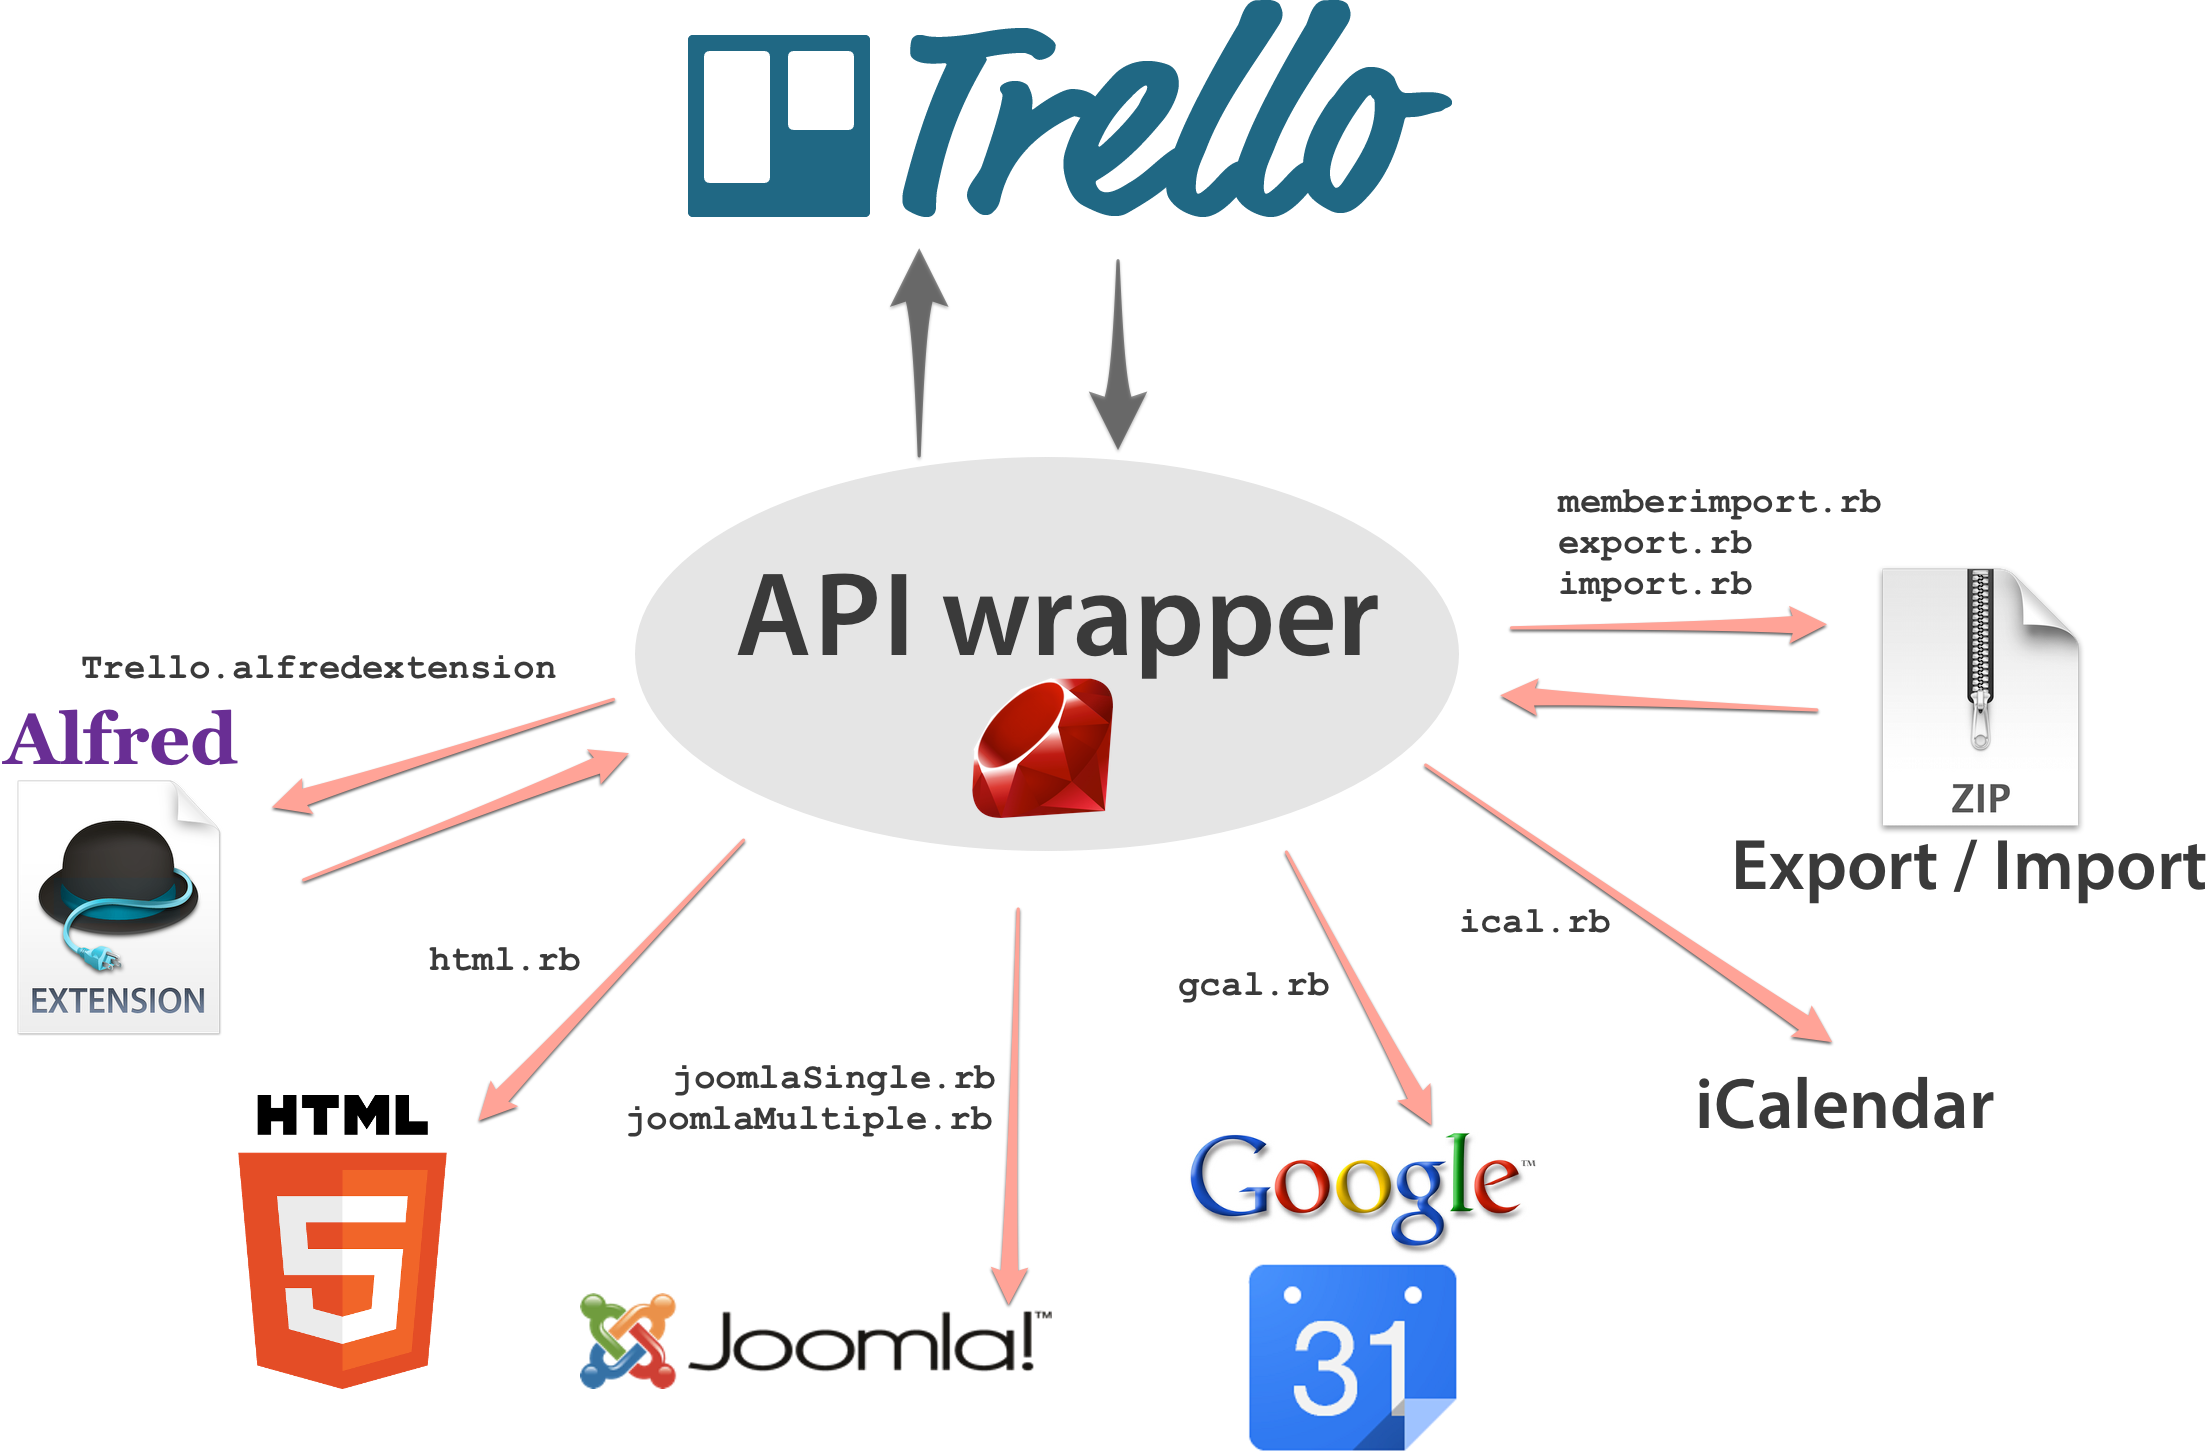
\includegraphics[width=\textwidth]{figures/api-wrapper}
\caption{Connections between Trello, the API wrapper and the actual features. \cite{ruby:icon}\cite{html:logo}\cite{joomla}\cite{google} }
\label{fig: api-wrapper}
\end{figure}

The API wrapper has also functions to pre-process data for Ruby. From a developers point of view, Trello is all about cards. Cards are the only things in Trello with real data, not just meta data. So if the task is so get a board from the API\index{API} it means to get the cards of the board. There is an API call to get all cards which are in a specific board. But with this call the developer doesn't get all information about the cards. So the API wrapper has to execute the API call for a single card to cummulate all information about all cards of the board. This is the function of the API wrapper to keep the actual script clean. So the developer can work with the data and hasn't to worry about determining them.

\section{Command Line Interface}\nomenclature{CLI}{Command Line Interface}\index{CLI}\index{Command-Line Interface}
Almost every script needs some informations. An information which every scripts need is key and token of the user which account should be used for the access to Trello. The scripts have to know which cards, lists and boards they have to look at. So these information has to be passed to the scripts, too. At first we set this information at the top of the script. But it emerged that it's very unpractical to hard code this in each script. So it would be impossible to use the same Ruby file with several Trello accounts. For every Trello account the user has to generate a dedicated file. The solution for this problem is a command-line interface (CLI). With a CLI the user can pass information to the script in a predefined format, so the script knows exactly what to do. For every other call the user can specify different information for one and the same script.

The Ruby class OptionParser\cite{ruby:optionparser} provides easy customisable command-line option analysis. The developer is able to specify its own options for each script. For this purpose a dedicated class is used. 
In order to let the actual script \emph{know} about the CLI arguments the developer has to require the respective CLI class with the command-line option definitions.

\begin{lstlisting}[style=bash, float=htb, caption=Example usage of a script with CLI., label=listing004]
ruby html.rb -c 4ffd78a2c063afeb066408b8
\end{lstlisting}

An example usage of a script with CLI would look like Listing \ref{listing004}. The \texttt{-c} is an comman-line option. If there is a string behind the option, like in this case, the string is a so called \emph{argument}. But there are command-line options which stand for its own. Those are called \emph{flags}. Flags are only for polar decisions.

\begin{lstlisting}[float=htb, caption=Definition of a command-line option, label=listing002]
# Trello list(s)
opts.on("-l", "--lists x,y,z", Array, "Ids of one or more Trello lists.") do |lists| (*@\label{line001}@*)
	options.lists = lists
end
\end{lstlisting}

Listing \ref{listing002} shows the definition of the option \texttt{-l} for passing one or more IDs of lists to a script. In Line \ref{line001} the word \lstinline{Array} casts the list argument to an Array object.

OptionParse provides an automated help option. If the user types 
\begin{center}
\texttt{ruby script.rb -h} 
\end{center}
he gets the explanation the developer wrote in the CLI class for this script with all possible options. This list ist automatically generated by the definitions of the command-line options like in Listing \ref{listing002}. It works with \texttt{-help} and \texttt{--help} instead of \texttt{-h}, too.

\begin{lstlisting}[style=bash, float=htb, caption=Output of the \texttt{-h} option., label=listing003]
Usage: ical.rb [options]
Select the input cards with -c, -l, -b or -a

Specific options:
 -a, --[no-]all         Set this if all due dates of all cards of all boards this user can see shall be used.
 -l, --lists x,y,z      Ids of one or more Trello lists.
 -b, --boards x,y,z     Ids of one or more Trello boards.
 -c, --cards x,y,z      Ids of one or more Trello cards.
 -k MANDATORY, --key    Your Trello key.
 -t MANDATORY, --token  The Trello token.
\end{lstlisting}

Listing \ref{listing003} shows the Output of \texttt{ruby ical.rb -h}. 
These are the basic CLI commands used by every script. For some scripts there are additional commands. They are explained in their respective sections.

\section{Export to HTML}\nomenclature{HTML}{Hyper Text Markup Language}

Used gems:
\begin{itemize}
	\item \texttt{erb}
	\item \texttt{json}
	\item \texttt{open-uri}
	\item \texttt{pp}
	\item \texttt{kramdown}
\end{itemize}

The \texttt{html.rb} script exports the data of one ore more cards to an HTML file. The resulting HTML file lists the cards one below another. The order is determined by the order in the command-line argument. If the command-line looks like listing \ref{listing005} the script will process the list with the id \texttt{4ffd78ff7f0c71780cc5aa1c} at first. That means in the HTML file are all cards in this list and below these the single card with the id \texttt{4ffd78a2c063afeb066408b8}.
Each card is displayed with all their information. This includes title, description, members, due date, labels, votes, checklists, comments and attachments.

\begin{lstlisting}[style=bash, float=htb, caption=Example for a \texttt{html.rb} call., label=listing005]
ruby html.rb -l 4ffd78ff7f0c71780cc5aa1c                 -c 4ffd78a2c063afeb066408b8
\end{lstlisting} 

Trello itself distinguishes between photos and other attachments. Normal attachments are linked under the description. Photos are embedded in the HTML code as thumbnails. The \texttt{html.rb} script does the same.

\subsection{Markdown}\index{Markdown}
Markdown is a small lightweight plain text formatting snytax, designed by John Gruber. It's designed for the use with blogs and CMS\nomenclature{CMS}{Content Management System}. In these use cases HTML is often too much. Markdown represents most of the features of HTML that are needed for writing. The designer of Markdown, had the goal that a text, written in Markdown, is still easy to read. John Gruber provides a software tool, written in the Perl programming language, that converts the Markdown formatted text to valid HTML. \cite{markdown}

\begin{lstlisting}[style=bash, float=htb, caption=Example for a text written in Markdown., label=listing006]
### iCloud:(*@ \label{line002} @*)

1.   Shared Photo Streams Now you can *share* just the **photos** you want, with just the people you choose. (*@ \label{line003} @*)
2.   Reminder

------------------------------- (*@ \label{line004} @*)

Here is an example of AppleScript:

    tell application "Foo" (*@ \label{line005} @*)
        beep
    end tell

![Apple logo](http://upload.wikimedia.org/wikipedia/commons/f/fa/Apple_logo_black.svg "Apple logo") (*@ \label{line006} @*)
\end{lstlisting}


\begin{lstlisting}[style=html, float=htb, caption=Listing \ref{listing006} converted to HTML., label=listing007]
<h3>iCloud:</h3>

<ol>
	<li>Shared Photo Streams Now you can <em>share</em> just the <strong>photos</strong> you want, with just the people you choose.</li>
	<li>Reminder</li>
</ol>

<hr>

<p>Here is an example of AppleScript:</p>

<pre>
	<code>tell application "Foo"
	beep
	end tell</code>
</pre>

<p><img alt="Apple logo" title="Apple logo" src="http://upload.wikimedia.org/wikipedia/commons/f/fa/Apple_logo_black.svg"></p>
\end{lstlisting}

 

Listing \ref{listing006} shows a small example of Markdown. The \lstinline{###} in line \ref{line002} is a header equal to \lstinline{<h3>} in HTML. The first list item of the ordered list in line \ref{line003} contains italic and bold words. In line \ref{line004} is a horizontal line. After a normal line of text a code block starts in line \ref{line005}. At the end in line \ref{line006} there is a picture with title and alt texts. After the conversion it looks like listing \ref{listing007} in HTML. The appearance, of course, depends on the used CSS on the respective websites. The appearance in Trello is like in figure \ref{fig:markdown-result}.

\begin{figure}[htb]
\centering
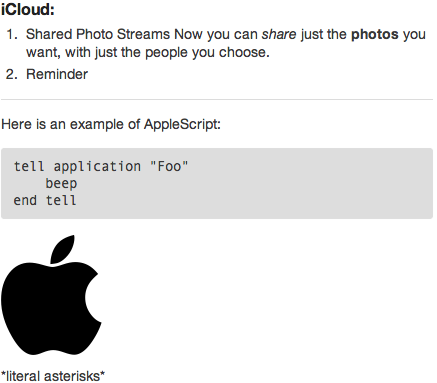
\includegraphics[scale=0.6]{figures/markdown-result}
\caption{The browser view of the HTML converted from the Markdown in listing \ref{listing006}}
\label{fig:markdown-result}
\end{figure}

Meanwhile Markdown became quite popular. Many blogging platforms support it, at least there are Markdown plug-ins for most platforms. Trello supports it in the description of cards. In the unlikely case that markdown reaches its limits inline HTML can be used. The only restriction ist, that HTML block-level-elements have to be separated to the previous and following Markdwon blocks.

For converting Markdown to HTML the gem kramdown is used. Figure \ref{fig:kramdown} decribes the convert options of kramdown. It converts to LaTeX and a special kramdown format, too. The kramdown format is an extended Markdown syntax. As input formats it accepts HTML and kramdown besides standard Markdown. \cite{kramdown} These additional features of kramdown might be useful for future approaches. To generate lists bibliographies for scripts, papers or books.

\begin{figure}[htb]
\centering
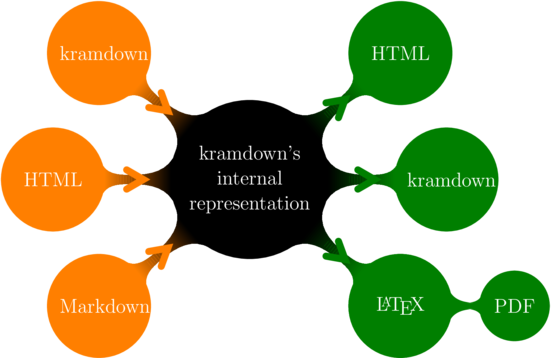
\includegraphics[width=\textwidth]{figures/kramdown}
\caption{Overview about kramdowns converting options. \cite{kramdown}}
\label{fig:kramdown}
\end{figure}

\subsection{Twitter Bootstrap Framework}\index{Twitter}\index{Bootstrap}

\subsection{HTML 5}\index{HTML!5}

\subsection{CSS 3 / LESS}\nomenclature{CSS}{Cascading Style Sheets}\index{CSS!3}

\subsection{ERB / Templating}\index{ERB}\index{Templating}

\section{One way sync to Google Calendar}\index{Google!Calendar}

\section{Export to iCalendar}\index{iCalendar}

\section{One way sync to Joomla}\index{Joomla}

\subsection{For every card an article}

\subsection{All cards in one article}

\section{One way sync to WordPress}\index{WordPress}

\section{Backup}\index{Backup}

\subsection{Export}\index{Export}

\subsection{Import}\index{Import}

\subsubsection{Filename option}
The \texttt{-n} (or \texttt{-name}) argument for this script stands for the filename of the backup\index{Backup} file which contains the  exported Trello data. With \texttt{-n} the user can specify a file to import. While processing the script first checks if the user has passed this argument. If not, it aborts. If the \texttt{-n} argument is given, the scipt proofes if the file is a ZIP\index{ZIP} file. For that it soesn't use the filename but the MIME\nomenclature{MIME}{Multipurpose Internet Mail Extensions}\index{MIME} type of the file.

\todo{listing design}
\begin{lstlisting}[float=htb, caption=Checking if the file has the MIME type \textquotedblleft application/zip\textquotedblright, label=listing008]
if `file -Ib #{@filename}`.gsub(/;.*\n/, "") != "application/zip"
	puts "ERROR: The backup\index{Backup} file has to be a ZIP\index{ZIP} file!"
	abort
end
\end{lstlisting}

	
In line 1 the \texttt{file -Ib \#\{\@filename\}} is a bash call for receiving the MIME\index{MIME} type of a file. Ruby executes it and with the gsub-Method it cuts the MIME part out of the received string. This shell script part in a ruby file is a bit dirty. But only for this small case it would be elaborately to use a seperate gem.

\todo{What's a MIME\index{MIME} type?}

\subsection{Member import}

